\documentclass[a4paper, 12pt]{article}
\usepackage{titling}
\usepackage{array}
\usepackage{booktabs}
\usepackage{enumitem}
\usepackage{graphicx}
\usepackage{hyperref}
\usepackage{amssymb}
\usepackage{listings}
\usepackage{color} %red, green, blue, yellow, cyan, magenta, black, white
\setlength{\heavyrulewidth}{1.5pt}
\setlength{\abovetopsep}{4pt}
\setlength{\parindent}{0pt}
\graphicspath{{.}}

\usepackage[margin=1in]{geometry}
\definecolor{mygreen}{RGB}{28,172,0} % color values Red, Green, Blue
\definecolor{mylilas}{RGB}{170,55,241}
% Must be after geometry
\usepackage{fancyhdr}
\pagestyle{fancy}
\fancyhf{}
\rhead{SEE Assignment 7}
\lhead{P.Lukin, E. Ovchinnikova}
\cfoot{\thepage}

\setlength{\droptitle}{-5em}

\title{Scientific Experimentation and Evaluation  \\
				Assignment: 7}
\author{Petr Lukin, Evgeniya Ovchinnikova}
\date{Lecture date: $7^{th}$ November 2016}

\begin{document}
%-------------------------------------------------------------------------------
\lstset{language=Matlab,%
    %basicstyle=\color{red},
    breaklines=true,%
    morekeywords={matlab2tikz},
    keywordstyle=\color{blue},%
    morekeywords=[2]{1}, keywordstyle=[2]{\color{black}},
    identifierstyle=\color{black},%
    stringstyle=\color{mylilas},
    commentstyle=\color{mygreen},%
    showstringspaces=false,%without this there will be a symbol in the places where there is a space
    numbers=left,%
    numberstyle={\tiny \color{black}},% size of the numbers
    numbersep=9pt, % this defines how far the numbers are from the text
    emph=[1]{break},emphstyle=[1]\color{red}, %some words to emphasise
    %emph=[2]{word1,word2}, emphstyle=[2]{style},
}

%-------------------------------------------------------------------------------


\maketitle

\section{Experiment setup}

After obtaining experimental data, we want to build a motion model using the following assumptions:
\begin{itemize}
\item effective speed and rotational speed of the robot is different from the commanded speed and can be modelled like $v_{effective} =k_v v+b_v $ , $\omega_{effective} =k_{\omega} v+b_{\omega} $.
\item additionally, robot motion is affected by random error that can be modelled by adding random values to speeds based on speed modules. 
\end{itemize}

In order to find effective speed coefficients, motion simulation was started for all 5 experiments. Cumulative error along the path was used as a cost function.

\lstinputlisting{effSpeedErr.m}

At first, optimization procedure were made to find effective speed coefficients with $\alpha$ set to zero. Next, obtained effective velocities were used in optimization procedure to find $\alpha$. Finally motion simulation was repeated to compare results.

\section{Experimental results}

\subsection{Experimental results for effective velocity}


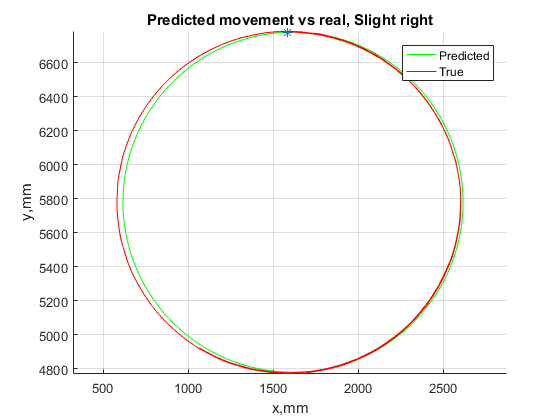
\includegraphics[scale = 0.8]{re.png}

Effective velocity parameters: $[k_v, b_v, k_{\omega}, b_{\omega}]$ = $[0.9503,~    1.1852,~    0.0002,~   -0.0001]$.

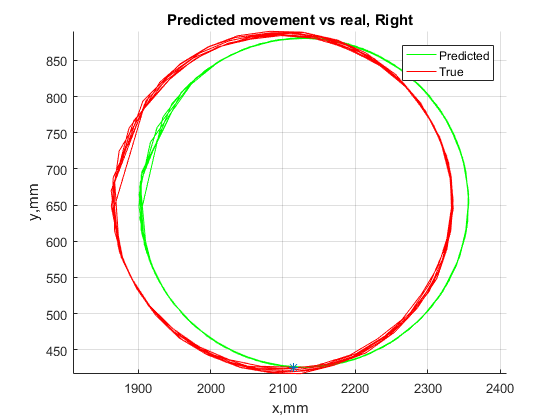
\includegraphics[scale = 0.8]{rre.png}

Effective velocity parameters: $[k_v b_v k_{\omega} b_{\omega}]$ = $[0.8064,~    2.0952,~    0.0013,~    0.0024]$.

They are really different for right movement.

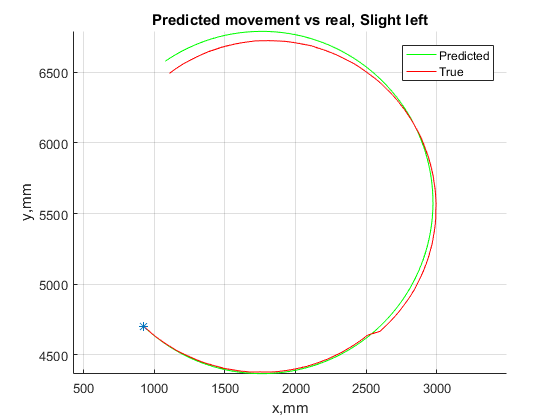
\includegraphics[scale = 0.8]{le.png}

Effective velocity parameters: $[k_v b_v k_{\omega} b_{\omega}]$ = $[0.9595,~    0.9849,~    0.0001,~    0.0004]$.

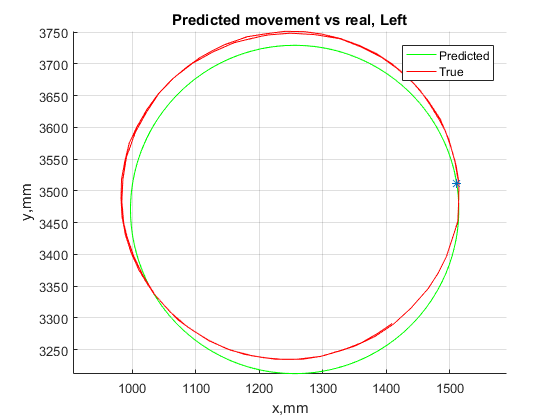
\includegraphics[scale = 0.8]{lle.png}

Effective velocity parameters: $[k_v b_v k_{\omega} b_{\omega}]$ = $[0.8374,~    0.9512,~    0.0005,~    0.0002]$.

In case of left movement, effective speed is not so different from the real one.

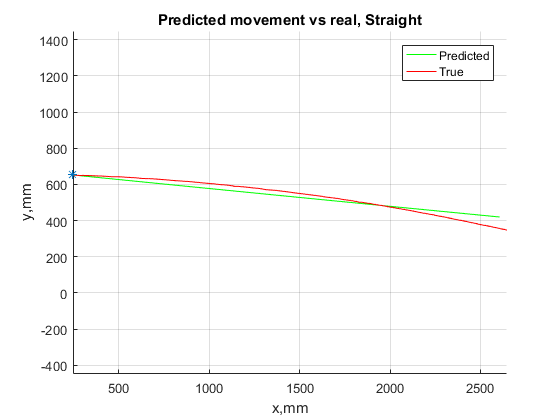
\includegraphics[scale = 0.8]{se.png}

Effective velocity parameters: $[k_v b_v k_{\omega} b_{\omega}]$ = $[0.9249,~    1.0867,~   -0.0002,~    0.0001]$.

Forward movement is most precise, but still there are some difference with given command.

Experimental results for effective velocity + $\alpha $

\subsection{Experimental results for effective velocity + $\alpha s$}

Alpha optimization algorithm is very sensitive to starting conditions and commanded speeds. Usually, it gives results that spoil all picture. The good set is $\alpha =  [1.40713612e-02,~~   6.03395470e-02,~~   0,~~   5.69003880e-02,~~   0,~~   0]$.

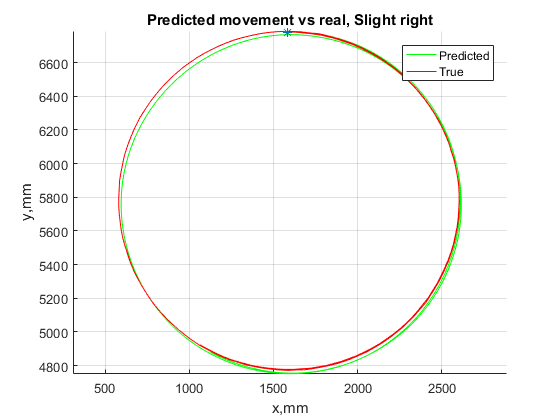
\includegraphics[scale = 0.8]{ra.png}



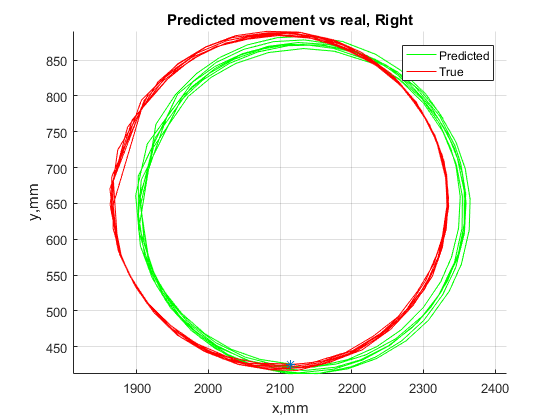
\includegraphics[scale = 0.8]{rra.png}




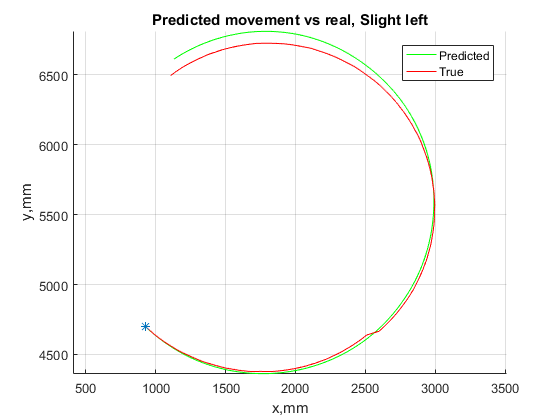
\includegraphics[scale = 0.8]{la.png}


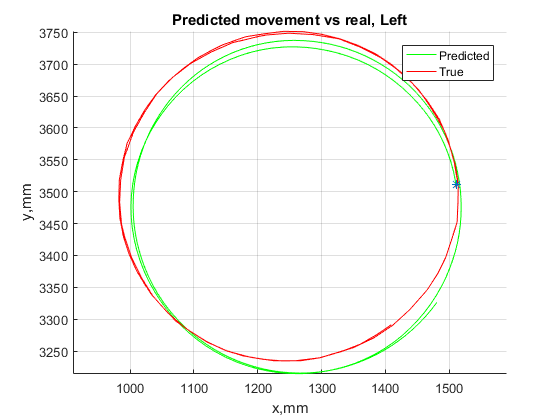
\includegraphics[scale = 0.8]{lla.png}

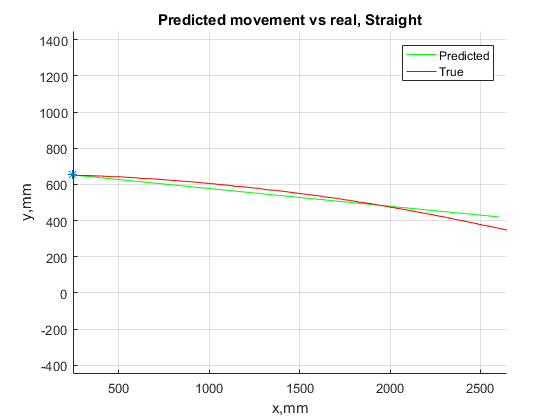
\includegraphics[scale = 0.8]{sa.png}

The figures show that precision of model with alpha only spoil the picture.

\subsection{Comparison of random and systematic error}

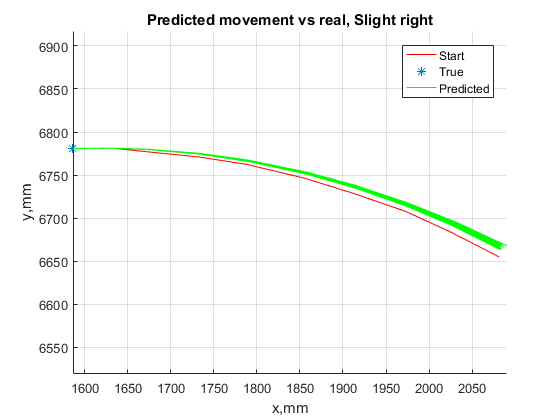
\includegraphics[scale = 1]{afan.png}

Only with small number of iteration steps, random error is comparable to systematic error.

\section{Conclusion}

The results can be concluded in a following way:
\begin{itemize}
\item For this particular robot and set of experiment systematic error is more important that random.
\item Random error has almost no influence in original model.
\item Actual desired and performed speed command is hard to measure in this setup.
\item Data was spoiled because experiments were made in 2 days.
\item More advanced procedure is needed to find systematic error.
\item Optimization procedures fall in local minima: starting point can change picture dramatically.
\end{itemize}



\end{document}
